\chapter{Methods}
\label{chap:methods}
In the design of a detector the theory must be supplemented by accurate models of the complex interactions in the radiation portal monitor to determine the performance.
Once the performance of a design has been determined a method must be chosen for how to optimize the design to  ensure the best use of the materials while meeting the performance criteria.
Three models of the detector physics are employed; two Monte Carlo based methods and one deterministic method.
The deterministic model, XSDRN \cite{XSDRNPM_2011}, solves a discretized one dimensional Boltzmann transport equation, and is described in \autoref{sec:XSDRNModel}.
Probabilistic models follow the path of individual neutrons with interactions based on the probability of a given event occurring.
Such codes are also known as Monte Carlo models, for which MCNPX (described in \autoref{sec:MCNPXModel}) and GEANT4 (described in \autoref{sec:G4Intro}) are well known examples.
MCNPX is employed for detailed neutronic modeling, while GEANT4 is employed for optical photon simulations and detailed energy deposition calculations.

The optimization of the detector is completed by a genetic algorithm using the XSDRN model to quickly simulate a large number of geometries.
Small perturbations on these geometries are then modeled with the MCNPX model to ensure that the results are accurate and that true convergence has been reached.
The genetic algorithm is introduced in \autoref{sec:GAIntro}.

\section{Pulse Height Discrimination}
\label{sec:PulseHeightDiscrm}
%%%%%%%%%%%%%%%%%%%%%%%%%%%%%%%%%%%%%%%%%%%%%%%%%%%%%%%%%%%%%%%%%%%%%%%%%%%
%                                                                         %
%                      Pulse Height Discrimination                        %
%                                                                         %
%%%%%%%%%%%%%%%%%%%%%%%%%%%%%%%%%%%%%%%%%%%%%%%%%%%%%%%%%%%%%%%%%%%%%%%%%%%
Generally, two methods are available for discrimination; 1) pulse shape discrimination and 2) pulse height discrimination.
In pulse shape discrimination the different decay times between the neutron and gamma pulses are exploited to develop a metric that allows for the classification of the pulse, and preforms best when the pulses are noticeably different.
Pulse height discrimination is based on setting a pulse height discriminator that acts as a partition between two classes of pulses.

A pulse height discriminator may be set by hardware electronics or by software.
A mathematical lower level discriminator (MLLD) is then introduced to clarify the determination of what discriminator setting will be necessary to achieve a given intrinsic efficiency criteria.
The intrinsic efficiency for a given MLLD is determined for a sample by first determining the photon fluence over the sample (usually by a MCNPX calculations, these calculations are explained in \autoref{chap:DetChar}).
The recorded spectra is then normalized the photon fluence to determine the count rate per incident photon per channel.
As the intrinsic efficiency is defined as the count per incident quanta of radiation, the spectra needs to be integrated from the channel number represented by the MLLD to the end of the spectra over the channels to determine the count rate.
By summing only the counts that are above the discriminator represented as the MLLD these counts are then discarded from the analysis.
A formulation of the MLLD is presented in \eqref{eqn:MLLDFormulation},
\begin{align}
	\epsilon_{\gamma,int}\left(MLLD\right) &= \frac{\int_{MLLD}^{\infty}p(x)dx}{\Phi}
  \label{eqn:MLLDFormulation}
\end{align},
where \definevar{$p(x)$}{spectra as a function of channel number} and \definevar{$\Phi$} is the incident gamma flux.
By computing the gamma intrinsic efficiency as a function of the MLLD, one only needs to find what MLLD corresponds to having a intrinsic efficiency of less than one in a million.

A sequence of polystyrene films (10\% by weight enriched LiF) were fabricated by Dr. Mabe and analyzed for their ability to achieve different gamma intrinsic efficiencies in the MLLD framework.
These measurements and calculations, presented in \autoref{fig:GammaIntEffMLLD}, demonstrate the utility of the MLLD.
This figure shows, as expected, that increasing the MLLD causes a lower intrinsic efficiency as counts below the MLLD are discarded.
Thicker films, where more energy is deposited and thus produce more photons, require higher MLLD settings in order to achieve the same level of discrimination as their thinner counter parts.
\begin{figure}
  \centering
    \includegraphics[width=\textwidth]{PS_intEffMLLD}
  \caption[Intrinsic efficiency achieved at various discriminator settings]{Gamma intrinsic efficiency versus the pulse height discriminator setting (MLLD) to achieve the corresponding level of discrimination in 10\% loaded polystyrene. It is observed that there is a change in the shape of the curves reflecting the increased fraction of energy deposition in thicker films relative to the thinner films.}
  \label{fig:GammaIntEffMLLD}
\end{figure}

A pulse height discriminator to achieve the necessary gamma discrimination will not be without cost, however, due to an overlap between the neutron and gamma pulse height distributions.
For example, the calculated gamma intrinsic efficiency for six polymeric films along with the neutron response of two of the films is shown in \autoref{fig:GammaIntrNeutronCounts},
In order to achieve an intrinsic efficiency of less than \num{1E-6} the MLLD must be set above 2,000 channels, discarding a large majority of the neutron counts.
It is observed that if the films are thin enough (less than \SI{150}{\um}) it is possible to have a significant count rate above the mathematical lower level discriminator necessary for the pulse height discrimination of one in a million.
This is seen by the \SI{50}{\um} film and the \SI{150}{\um} film having the tail of their neutron spectra above the pulse height discriminator necessary for an intrinsic efficiency of \num{1E-6}.
\autoref{tab:FractionCRGamma} shows the fraction of neutron count rate that is above the MLLD necessary for $\epsilon_{int,\gamma n} \le \si{1E-6}$.
Films less than \SI{50}{\um} have over 16\% of the counts above the necessary discriminator setting, while thicker films have have a factor of 10 less.
\begin{figure}[ht]
    \centering
    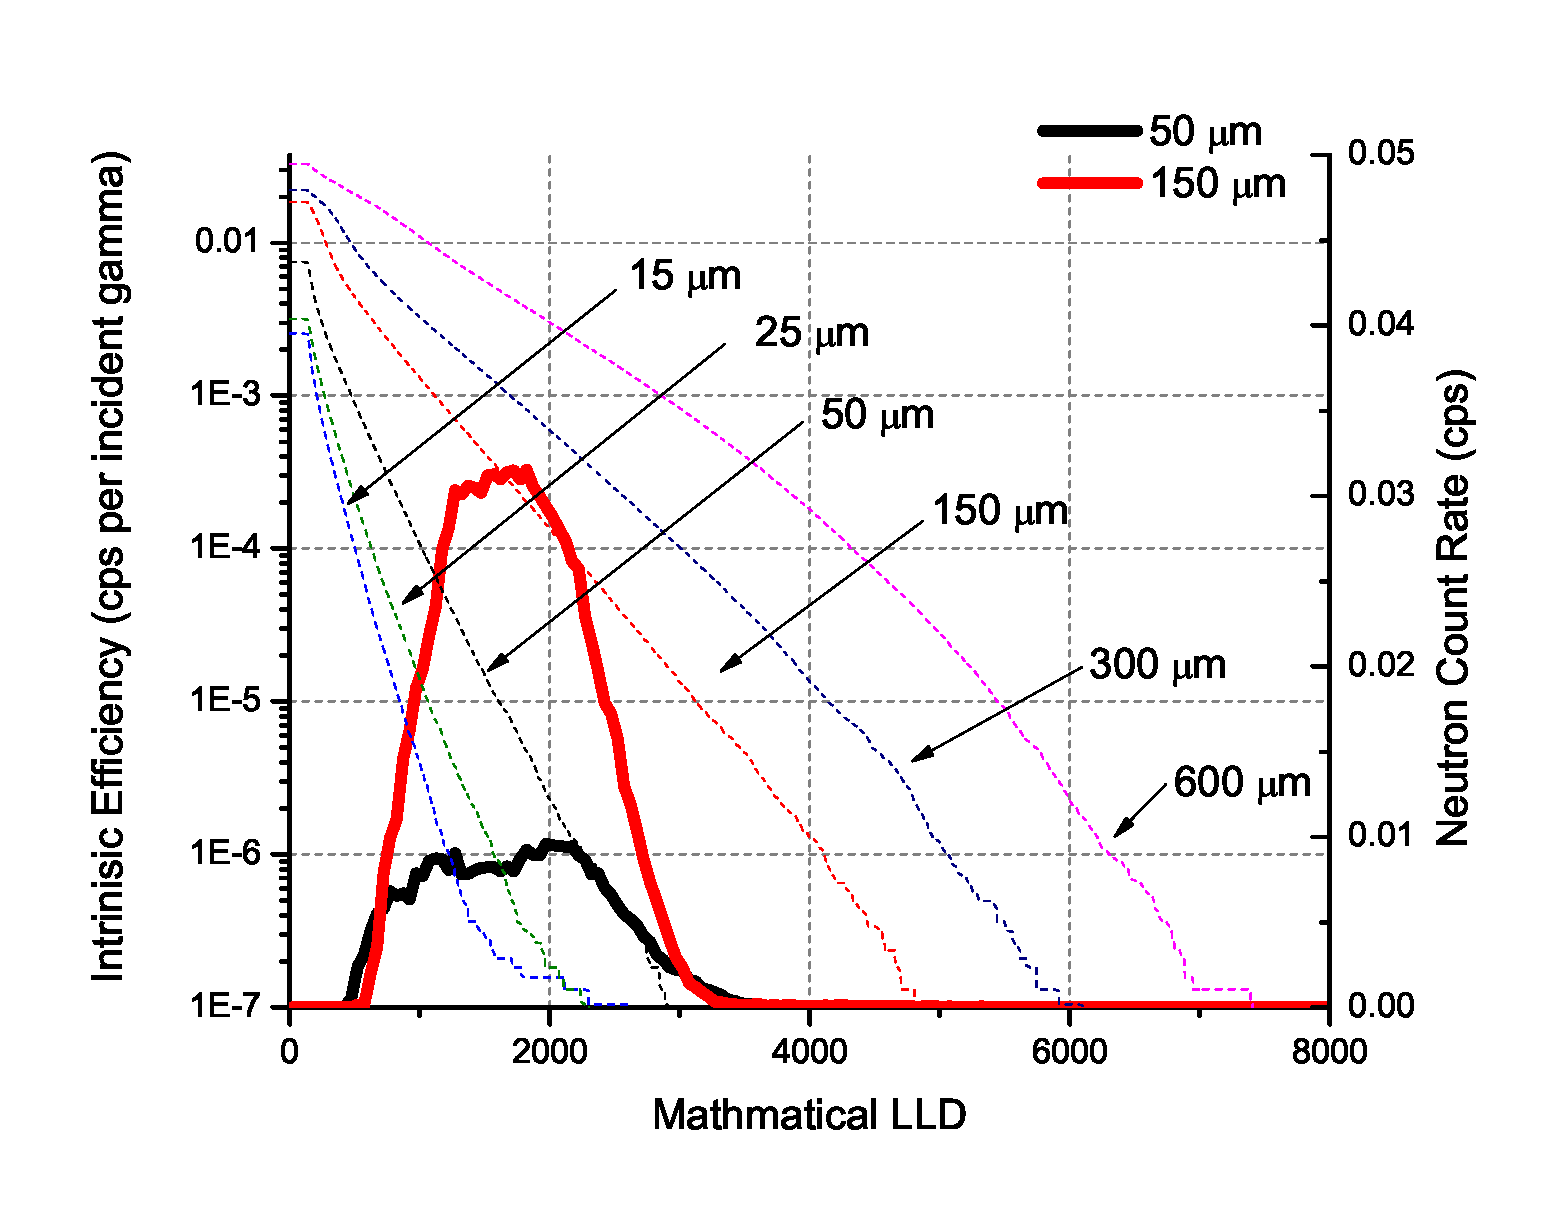
\includegraphics[width=\textwidth]{PS_IntEff_LiF20_PPO5}
    \caption[PS Gamma intrinsic efficiency and neutron count rate]{Gamma intrinsic efficiency (dashed lines) plotted against neutron counts (solid). The gamma spectra has been normalized by the number of incident photons upon the sample, while the neutron spectra has not. The material is polystyrene loaded with 10\% \iso[6]{LiF}.}
    \label{fig:GammaIntrNeutronCounts}
\end{figure}
\begin{table}
    \caption{Fraction of Neutron Count Rate Above Discriminator Setting in 10\% loaded polystyrene}
	\centering
	\begin{tabular}{c | c}
	Thickness & Neutron Fraction \\
	\hline
	\hline
	\SI{15}{\um} & 0.21 \\
	\SI{25}{\um} & 0.30 \\
	\SI{50}{\um}  & 0.16 \\
	\SI{150}{\um}  & 0.009 \\
	\SI{300}{\um}  & 0.002 \\
	\SI{600}{\um}  & 0.002 \\
	\end{tabular}
  \label{tab:FractionCRGamma}
\end{table}
In addition it is observed in \autoref{fig:GammaIntrNeutronCounts} that for neutrons, thicker films only enhance the resolution of the film and do little to increase the light yield, as most of energy from a neutron event is captured in the film.


\section{GEANT4 Modeling}
\label{sec:G4Intro}
GEANT4 is a free toolkit for the simulation of particles as they travel through matter\cite{agostinelli_geant4simulation_2003}.
In general two types of applications were authored with the GEANT4 toolkit; ranges along with energy deposition and light transport.
All of the applications shared a common electromagnetic physics list based on the Livermore data set, and a cross section driven hadron physics list was used for the neutron interactions.
Ions were transported with the general ion physics list which contains detailed alpha and triton models.
Optical photons were transported with the default Optical Photon physics list.
More details on the GEANT4 toolkit may be found in \autoref{chap:G4Intro}.

\subsection{Energy Deposition Simulations}
\label{sec:EnergyDeposition}
The GEANT4 toolkit has the ability to track the energy deposition in different materials as well as the tracking of electrons to a least \SI{1}{\keV}\cite{agostinelli_geant4simulation_2003}.
It is proposed to represent the detector geometry as a single layer of neutron absorbing thin polymeric film mounted on top of a non-scintillating material (PMMA).
For simplicity, the initial events for runs will be chosen by setting up a particle gun for thermal (\SI{0.025}{\eV}) neutrons upon the detector and for both gammas resulting from a \iso[60]{Co} decay.
\begin{figure}
  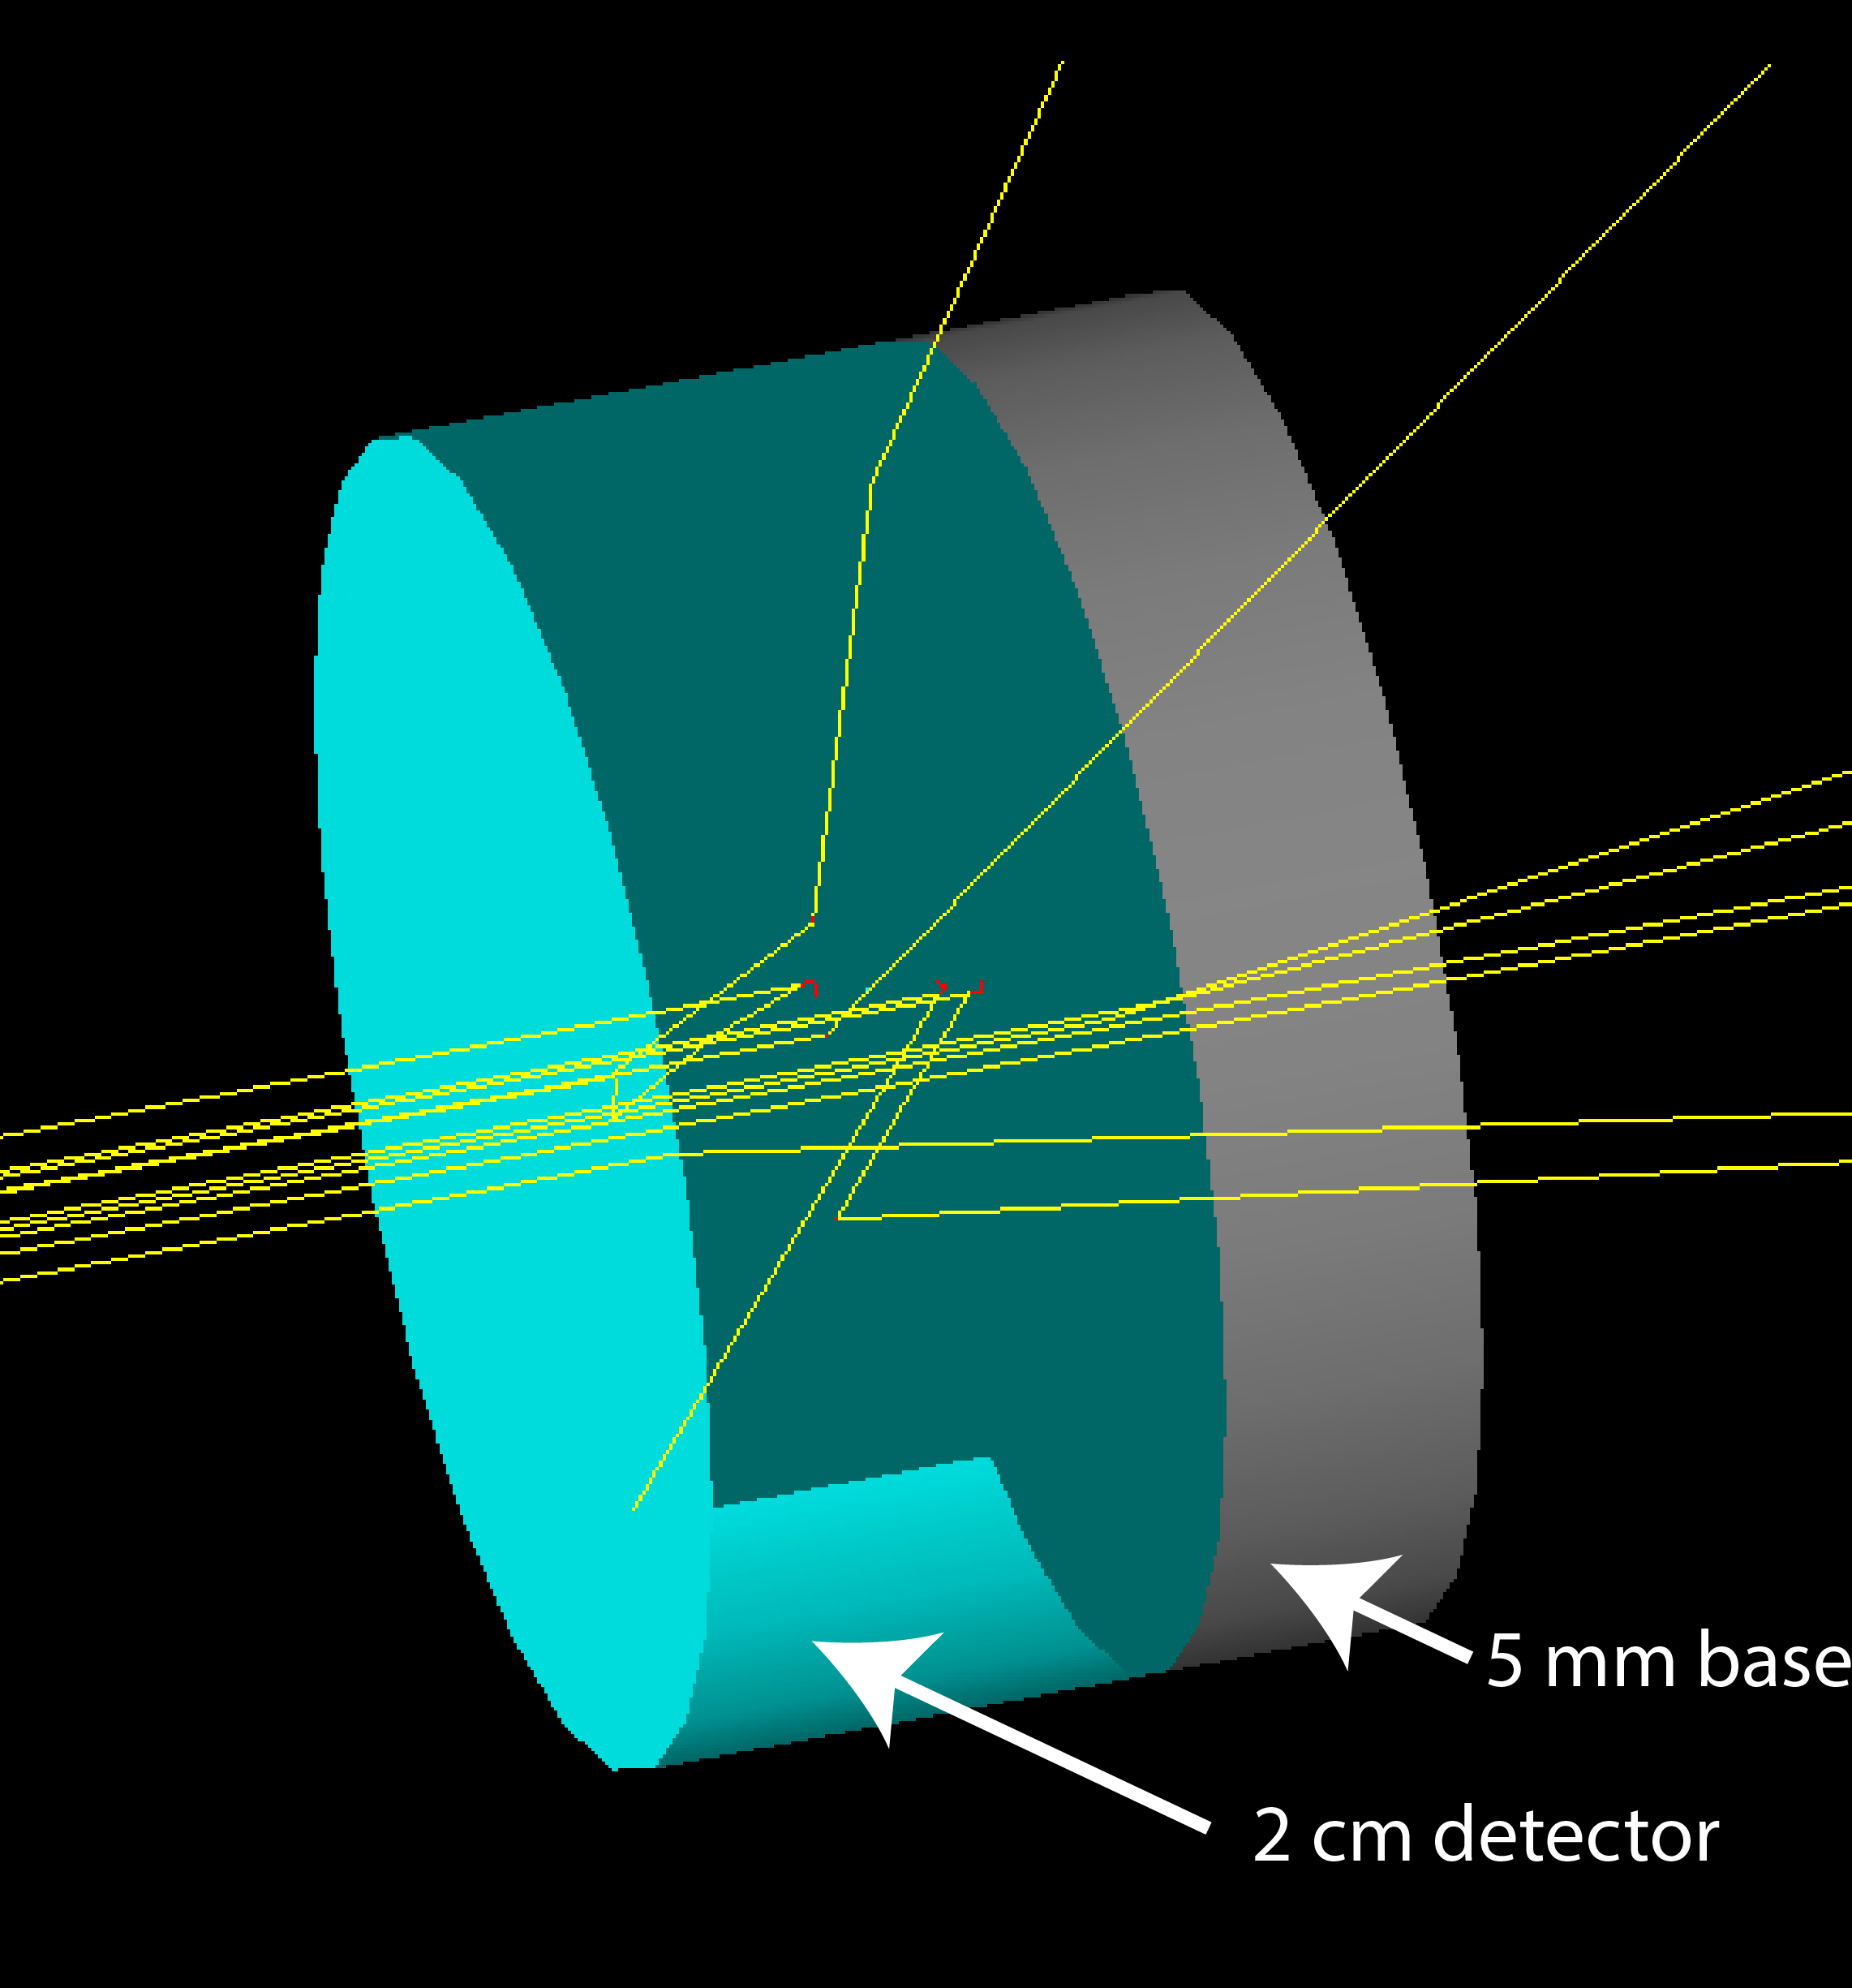
\includegraphics[width=\textwidth]{GEANT4AnnotatedGeo_EnergyDepEvent}
	\caption[GEANT4 Energy Deposition Geometry]{GEANT4 Geometry for the Simulation of Energy Deposition. What is shown are 10 photons from a \iso[60]{Co} source impingement upon a \SI{2}{\cm} thick detector.  The photon tracks are shown in yellow, while the electron tracks are shown in red.}
	\label{fig:EDepSimGeo}
\end{figure}
It is expected that the the Livermore data-driven parameterized electromagnetic physics will be necessary to calculate the ionizing energy deposition, extending the standard electro-magnetic physics down to \SI{1}{\kilo\eV}.
The neutron interactions will be simulated with a hadronic modules, using the \verb+HP+ flavored modules to use the ENDF cross sections to calculate the interaction rates.

\subsubsection{Energy Deposition Validation}
The validation of this GEANT4 simulation was completed by reproducing the single collision energy loss in water as well as comparing  the spectral shapes and averages of simulated and measured spectra.
The reproduction of the single collision energy loss will ensure that the electron physics are implemented correctly, while the simulation of the polymeric film energy deposition allows the user to gain confidence that the correct tracking and binning analysis has been implemented.

The simulation was validated by reproducing the single collision energy loss for water as well as comparing spectra shapes and averages of simulated spectra to the measured spectra.
The single collision energy loss spectra for water that was simulated is shown in \autoref{fig:SingleCollisionELossWater}.
In general there was excellent agreement between the simulated energy spectra and a previously published spectra\cite{turner_comparative_1982}, with the simulated spectra having much better resolution than the reference did not.
It is thought that this is due to the water model in GEANT4 having better cross sections than the previously published spectra.
\begin{figure}[ht]
  \centering
  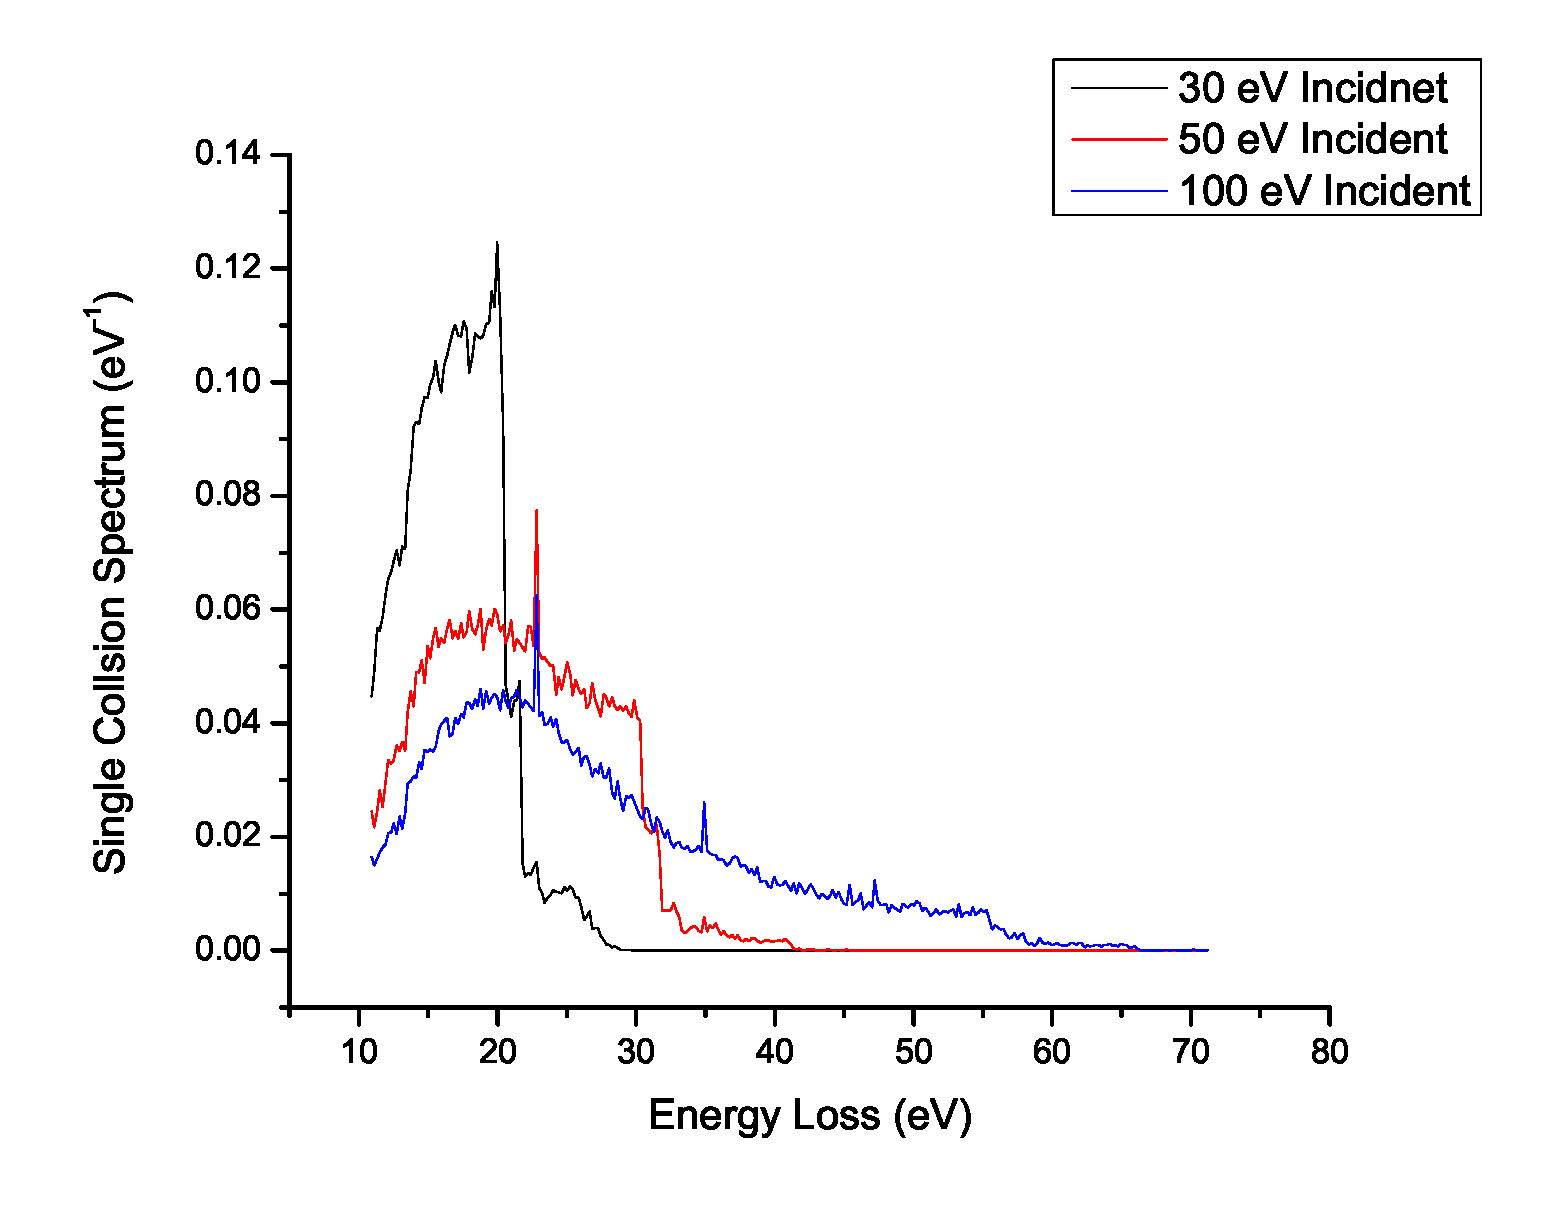
\includegraphics[width=\textwidth]{SingleCollisionEnergyLoss_300bins}
  \caption{Single Collision Energy Loss of Water. The simulated energy spectra matches that of Turner\cite{turner_comparative_1982}.}
	\label{fig:SingleCollisionELossWater}
\end{figure}

The validity of the GEANT4 simulation is determined by comparing the spectra shapes of measured spectra to simulated energy deposition.
Example gamma simulated spectra are shown in \autoref{fig:G4SimulatedEDep}, where for thin films there is an almost linear increase in the spectra endpoints with film thickness.
The simulated energy deposition per incident photon from a \iso[60]{Co} source and the measured pulse height spectra from the \iso[60]{Co} irradiator per incident photon can be compared by finding a calibration between them, in this case the Compton edge of a thick sample.
The measured Compton edge of a \SI{1}{\mm} film can then be correlated with the simulated energy, as shown in \autoref{fig:spectraComparisonGamma}.
The energy of this feature on the measured spectra was then compared to the energy on the simulated spectra, with all of the values being within 10\%.
\begin{figure}
	\centering
    	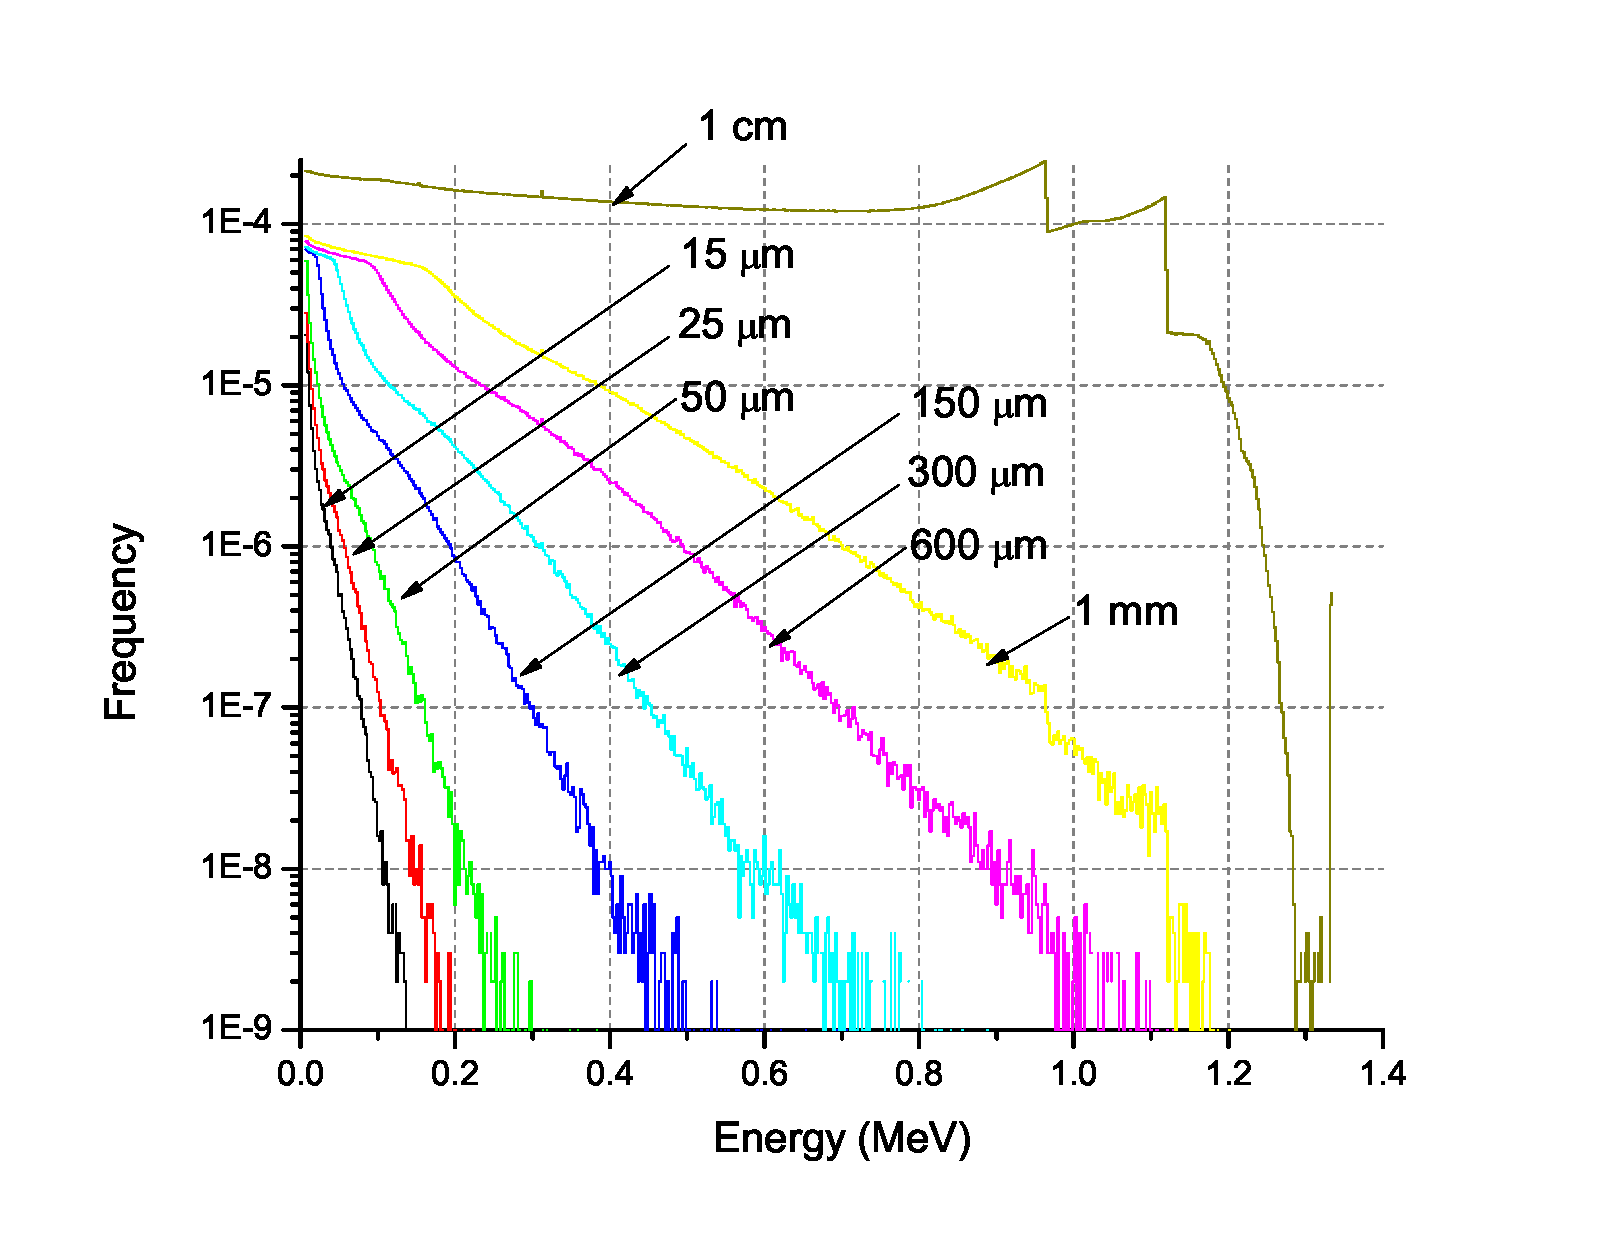
\includegraphics[width=\textwidth]{PS_EDepSim_Co60}
	\caption[GEANT4 Simulated Gamma Spectra in PS]{GEANT4 Simulated Energy Deposition}
	\label{fig:G4SimulatedEDep}
\end{figure}
\begin{figure}
	\centering
   	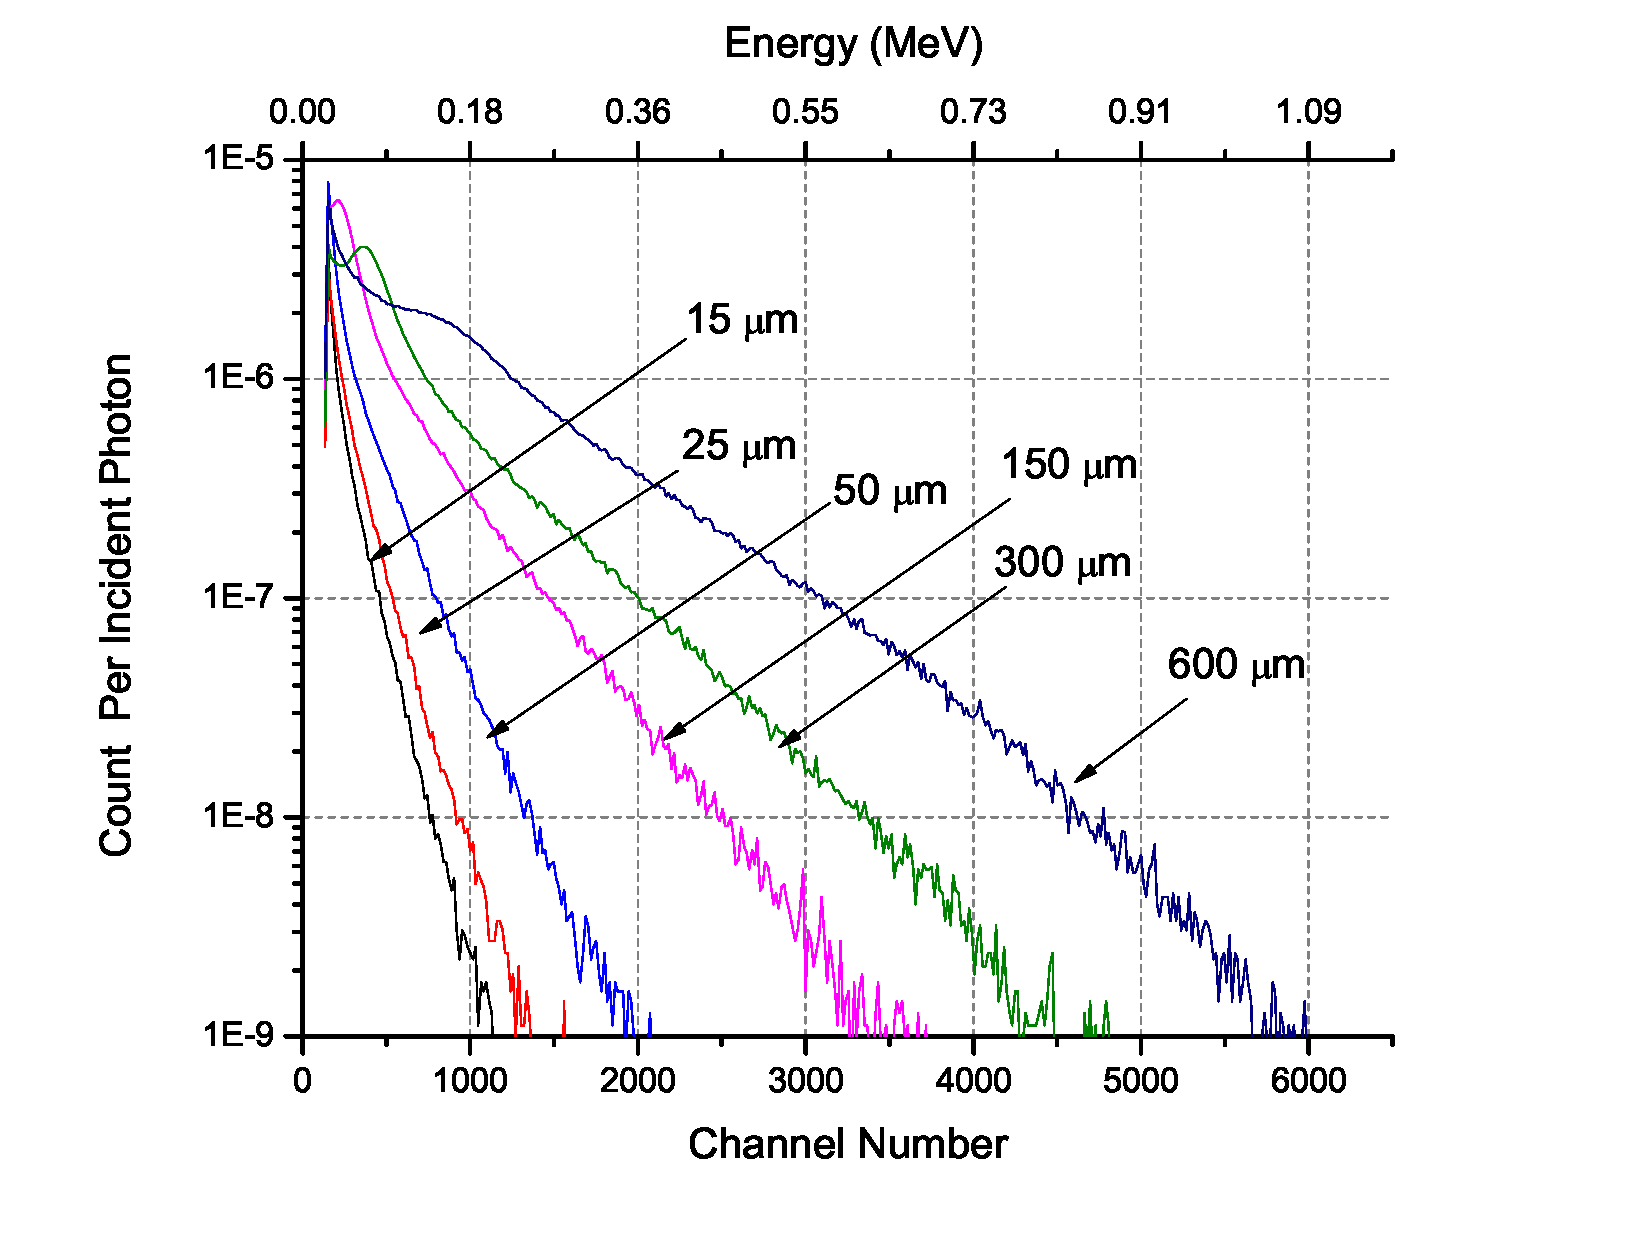
\includegraphics[width=\textwidth]{PS_GammaCR-Binned-FluxNorm_20LiF_5PPO}
	\caption{Comparison of the energy deposition and binned pulse height spectra for validation. The spectra have the same shape, indicating agreement. The fabricated films greater than \SI{600}{\um} were of poor optical quality and therefore their results are not shown.}
	\label{fig:spectraComparisonGamma}
\end{figure}

A direct comparison between the simulated average energy deposition and pulse height are shown in \autoref{fig:EDepLightYieldNeutron} and \autoref{fig:EDepLightYieldGamma}. 
The average energy deposition is shown on the left axis and the average light yield (pulse height) on the right axis.
The largest amount of energy that can be deposited in the neutron interaction is \SI{4.78}{\MeV}, which is approached after \SI{200}{\um} in both the measurement and simulations.
This asymptotic behavior is not observed for the gamma spectra.
\begin{figure}
	\centering
    	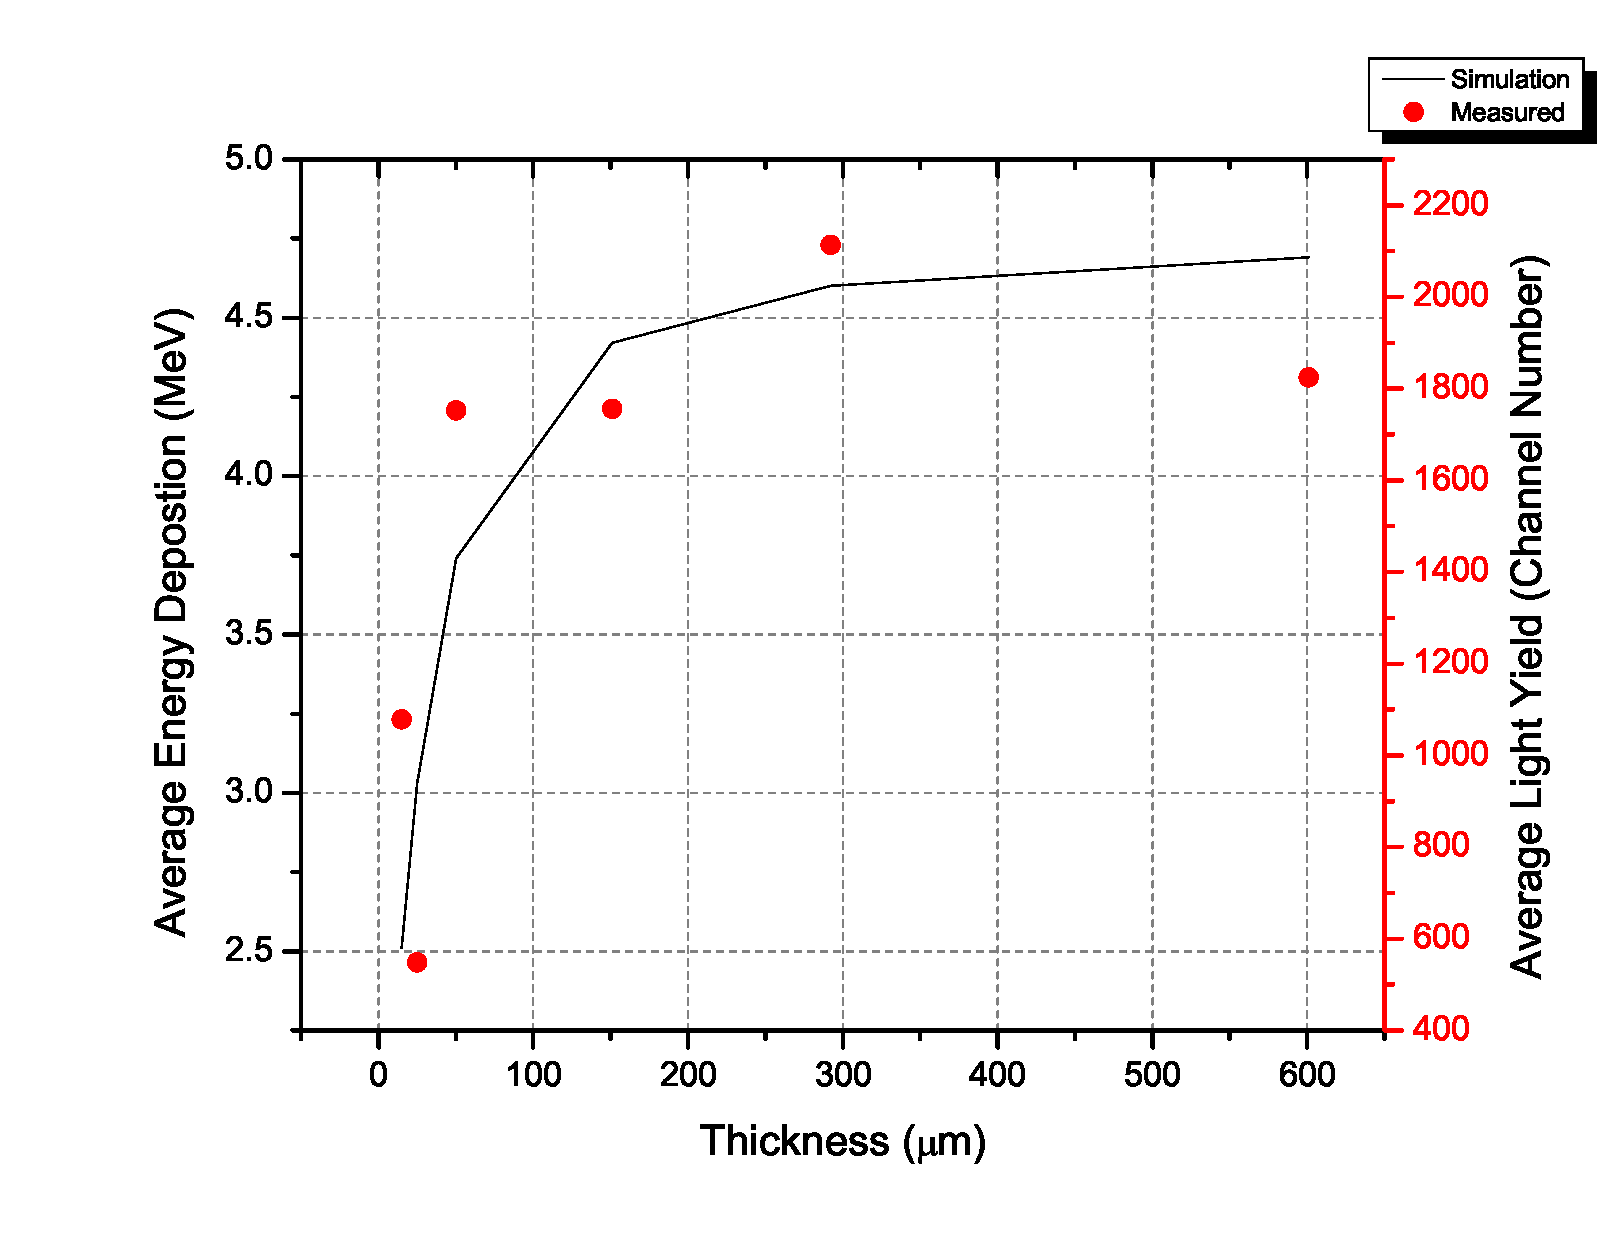
\includegraphics[width=\textwidth]{G4EDep_LightYield_Neutron}
	\caption[Average Light Yield and Energy Deposition for neutron interactions in PS]{Average energy deposition and measured light yield for neutron interactions. The solid lines are calculated values and the red dots are measurements.}
	\label{fig:EDepLightYieldNeutron}
\end{figure}
\begin{figure}
	\centering
    	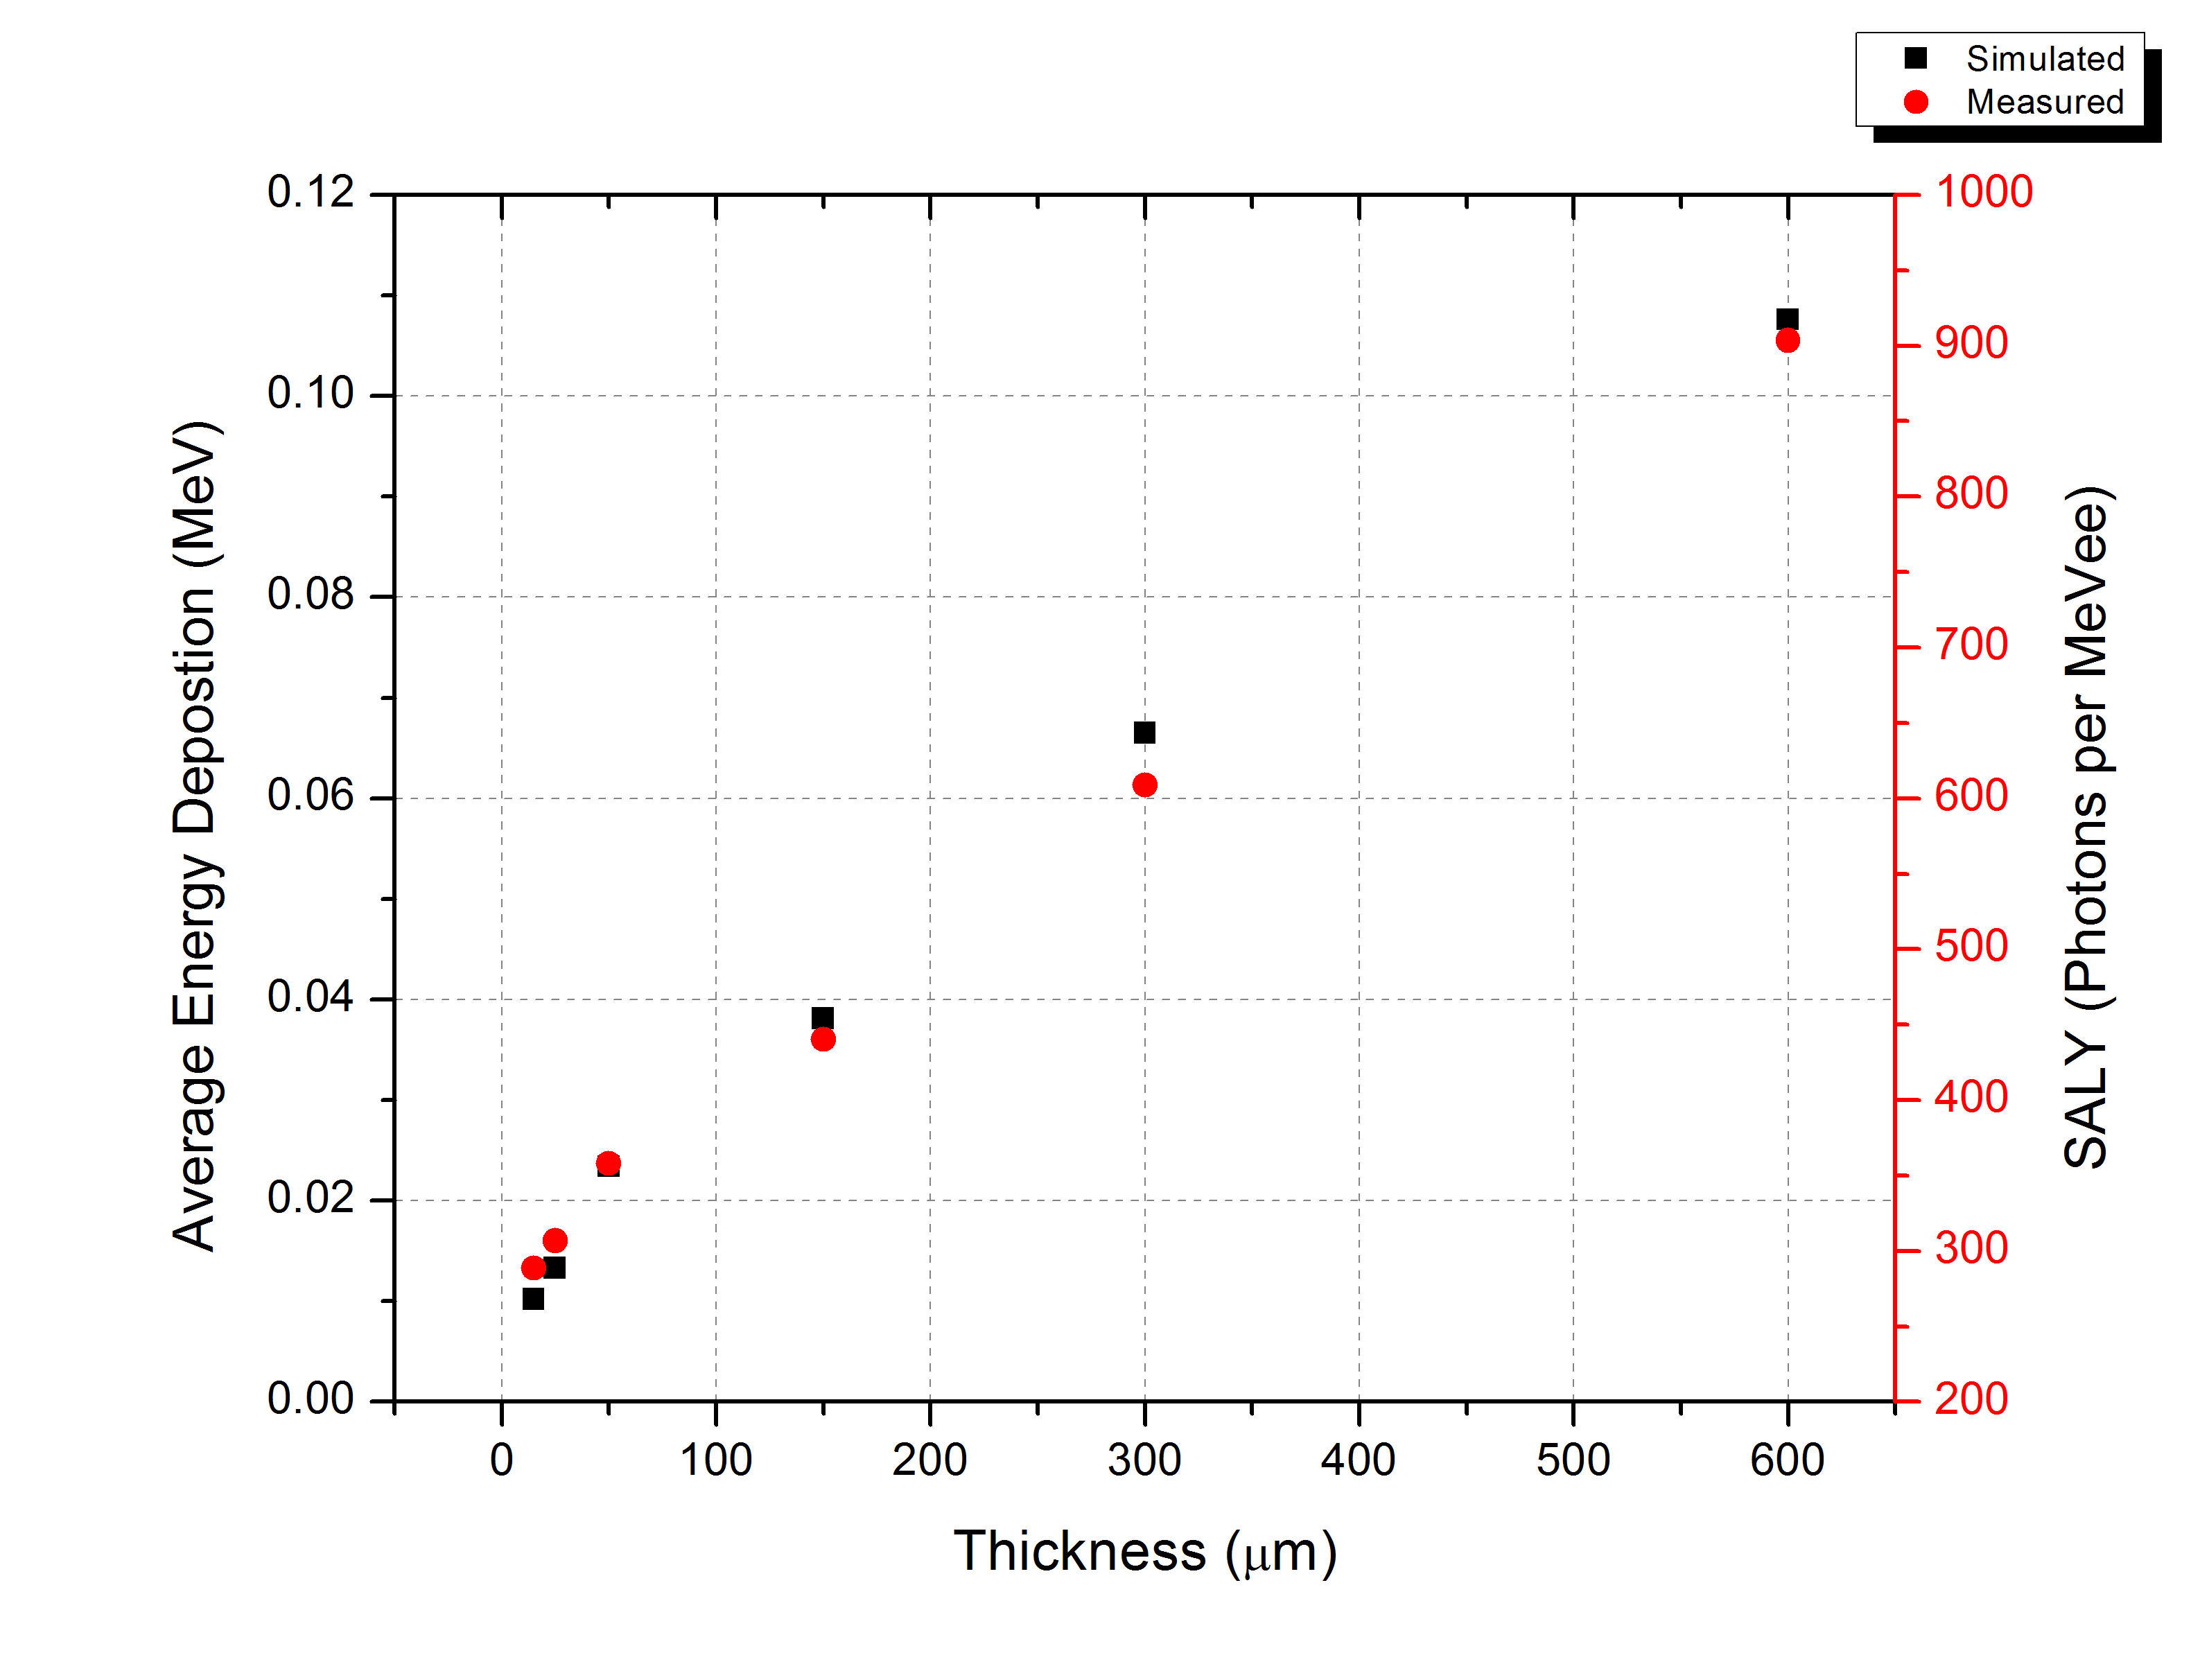
\includegraphics[width=\textwidth]{G4EDep_LightYield_Co60}
	\caption[Average Light Yield and Energy Deposition for Gamma interactions in PS]{Average energy deposition and measured light yield for \iso[60]{Co} interactions. The solid lines are calculated values and the red dots are measurements}
	\label{fig:EDepLightYieldGamma}
\end{figure}

\subsection{Optical Photon Simulations}
\label{sec:OpticalPhotonSims}
Photons are considered to be optical photons in the GEANT4 model when the wavelength of the photon is much greater than atomic spacing to allow for their wave-like nature.
Optical photons were simulated in GEANT4 by creating an optical material property for each of the optical materials.
In general this involves setting the scintillation yield of the material, the resolution of the material, the optical photon absorbance of the film, the decay time, and the Birks parameter of the material to simulate the light quenching of the material.
Scattering at the boundary between two surfaces can be  handled by the UNIFIED model for Optical Surfaces, by the use of look up tables based on the measured data values \cite{5485130}, or simply based on the index on Snell's law.
For this work a look up table model was employed.


\subsection{Optical Photon Validation}
\label{sec:OpticalPhotonValidation}
The GEANT4 optical photon model was verified by measuring a detector and then simulating a similar detector in the GEANT4 toolkit. 
The comparison of the simulated entire  detection mechanisms (including the energy deposition, scintillation, and optical photon collection) to the a measured value provides confidence in the entire model; however, it should be noted that a validation of this type could allow for individual errors to miraculously cancel each other out.
Two cases where considered for the validation: 1) a sample mounted onto a PMT and 2) fabricated layered detectors that where  \SI{10}{cm} by \SI{15}{cm} by \SI{6}{cm} .
The single sample mounted on the PMT was used to establish the Birks constant for the material, and the fabricated layered detectors measurements were used to provide confidence of the ability to simulate a large scale detector system.

A single sample mounted on a PMT provides a simple geometry to validate the parameters used in the light transport simulations. 
The geometry consist of a sample mounted with a thin layer of optical grease to the PMT, and the entire assembly is wrapped with teflon grease.
This mimics the measurement of a sample mounted on a PMT, expect for the efficiency of the photocathode is not considered.

It should be noted that the Birks constant greatly impacts the number of optical photons generated and subsequently detected.
For GS20 a Birks constant of \SI{0.1}{\mm\per\MeV} produced 1,300 photons per neutron, while a Birks constant of \SI{0.01}{\mm\per\MeV} produces 6,900 optical photons per neutron.
Birks constants greater than \SI{0.01}{\mm\per\MeV} produce marginal increases in the number of optical photons produced; for example 8,600 photons per neutron were produced for a Birks constant of \SI{0.0001}{\mm\per\MeV}.
If agreement between the simulated and measured c


\section{MCNPX Modeling}
\label{sec:MCNPXModel}
% MCNPX Model of the interaction rate
The performance of films is simulated in MCNPX, a Monte Carlo transport code\cite{pelowitz_mcnpx_????}.
The geometry is as in the PNNL reports, namely a nano-gram of \iso[252]{Cf}  encased in \SI{0.5}{\cm} of lead and \SI{2.5}{\cm} of HDPE. 
The size of the RPM8 is \SI{12.7}{\cm} deep, by \SI{30}{\cm} wide and \SI{2}{\m} tall.
The interaction rate, $I_{\text{sim}}$ provides the total number of simulated neutron interactions in the detector and is calculated using the a cell flux tally in MCNPX and a tally multiplier card.
The reaction rate $\iso[6]{Li}\left(\text{n},\text{t}\right)\alpha$ can be calculated by then applying the appropriate input for the FMn card and using an F4 card to calculate $\phi(E)$.
This is in accordance with the direct evaluation of the PNNL criteria, which require a absolute neutron count rate of \SI{2.5}{count\per\second\per\nano\gram\iso[252]{Cf}}.
Note that in this calculation the source strength is set to be \SI{1}{\nano\gram} \iso[252]{Cf}, which has a neutron emission rate of \SI{2.3E3}{neutron\per\second}.
\begin{align}
  \label{eqn:RPM8InteractionRate}
  I_{\text{sim}} &= S_0 I \\
  &= \SI{2.3E3}{neutron\per\second} I
\end{align}



\section{XSDRN Modeling}
\label{sec:XSDRNModel}
% XSDRN Model of the RPM
The XSDRN model was a simplified model of the RPM along an axis through the midpoint of the RPM.
A $S_n$ of 16 was used for the quadrature, and convergence for the flux was set at \SI{1E-7} for the inner iterations.
Only two types of materials were simulated in the XSDRN calculation; a detector material containing the \iso[6]{LiF} and a moderating material of polystyrene.
A 44 group neutron cross sections of each of these materials were processed using NITWAL \cite{NITAWL_2011} (without any resonance regions) assuming an infinite, homogeneous medium for simplicity.
The XSDRN model consisted of a multi-group isotropic boundary source on the left most boundary on the RPM, with the values for this flux calculated by an MCNPX simulation.
A MCNPX calculation was used to determine the neutron flux incident upon the left most side of the RPM, and then this flux was input as the surface boundary flux condition in XSDRN.
The number of neutron absorptions was calculated using an activity flag in the XSDRN model.
The fitness function for this model was implemented as the activity normalized the number of detector layers.
The number of layers was chosen as the normalization factor instead of the actual mass of absorber to allow for different film compositions to be simulated more readily.

The comparison between the MCNPX simulation and the XSDRN is shown for some of the samples in \autoref{tab:10GenomeXSDRNMCNPXCompare} and \autoref{tab:20GenomeXSDRNMCNPXCompare}, where the change in rank is computed by rank of the MCNPX model versus the rank of the XSDRN model.
It is observed that the XSDRN model preformed fairly closely to the MCNPX model, but tended to over predict and favor geometries that had repeated layers and clusters.
This was very noticeable when the geometries started with a neutron absorber layer this is attributed to the breakdown of the diffusion equation in a strongly absorbing medium near a source.
Some stratification of the results were also observed, leading to the conclusion that the XSDRN calculations should only be used as a general guide.
More details are available in the simulation code base, summarized in \autoref{sec:garpm8opt}.
\begin{table}
  \caption[10 Genome Length RPM Model]{10 Genome Length RPM Model Interactions rates}
  \label{tab:10GenomeXSDRNMCNPXCompare}
  \begin{tabular}{c c | c c | c}
    \toprule
    Genome & Activity & Interaction Rate & Rank Change \\
    \midrule
  0011010000& 9.30 &  3.82 & $\downarrow$ 13 \\
  0110100000 & 10.50  &  3.81 & 0 \\
  0101010000 & 10.12  & 3.79 & $\downarrow$ 7 \\
 0101100000 &  & 3.79 & $\downarrow$ 1\\
  0011100000 & 9.63 &  3.77 & $\downarrow$ 3 \\
    \bottomrule
  \end{tabular}
\end{table}
\begin{table}
  \caption[20 Genome Length RPM Model]{20 Genome Length RPM Model Interactions rates}
  \label{tab:20GenomeXSDRNMCNPXCompare}
  \begin{tabular}{c c | c c | c}
    \toprule
    Genome & Activity  & Interaction Rate & Rank Change \\
    \midrule
  00100101000000000000 & 7.77 & 3.79 & $\downarrow$ 19 \\
  00011000100000000000 &  & 3.78 &  \\
  00011000010000000000 &  &  3.76 &  \\
  00110001000000000000 &  &  3.69 & $\downarrow$ 15\\
  01011010010000000000 & 23.46 & 3.66 & $\uparrow$ 1\\
    \bottomrule
  \end{tabular}
\end{table}


\section{Genetic Algorithm Introduction}
\label{sec:GAIntro}
Genetic algorithms provide a search technique analogous to biological evolution in which instead of searching from general to specific solutions, or from more simple to complex, genetic algorithms generate solutions by mutating and combining parts of the best previously known solutions.
At each step in the search for the best solution a collection of solutions called the current \textit{population} is refined by replacing members with solutions representing the offspring of the best individuals.
The goals is then to find the best solution to the problem as determined by some criteria, called the \textit{fitness function}.
The genetic algorithm typically consist of four tasks: creating an initial population, evaluating that populations fitness, selecting members of the current population to breed, and then applying genetic operators to the selected members to breed the new population. 
This is completed until either a maximum generation is reached or the desired fitness is achieved, as shown in \autoref{alg:GAOutline}.
\begin{algorithm}
  \caption{Genetic Program Outline}
  \label{alg:GAOutline}
  \begin{algorithmic}
    \WHILE{$error>goal$}
      \FORALL{$t\in F$}
        \STATE{Compute fitness}
      \ENDFOR
      \FORALL{$t\in F$}
        \STATE{Choose individuals based on fitness}
      \ENDFOR
      \STATE{Select individuals for next population}
      \STATE{Crossover selected individuals}
      \STATE{Mutate selected individual}
    \ENDWHILE
  \end{algorithmic}
\end{algorithm}

\subsection{Problem Representation}
The thickness of the RPM  (\SI{12.7}{\cm}) was divided into slices, where each slice could be either a detector slice or a moderator slice.
These slices of detector material (represented as a \verb+1+) or moderator material (represented as a \verb+0+) were append into a sequence.
This sequence of one's and zero's (or bit string) then completely represented the geometry of the RPM and formed the basis for all possible solutions to the optimization problem.
For example the sequence \verb+0001110010+ would represent a detector that had three moderator slices, three detector slices, another two moderator slices, and a final detector slice before a single moderator slice as the reflector.
In terms of genetic algorithms the set of all possible solutions is referred to as the \textit{genome}.
The length of the genome is thus the number of slices in the geometry, where a higher length genome allows for a more complicated geometry.
The initial population for the genetic algorithm was initialized to be random bit strings with equal probability of a slice being a detector slice or moderator.

\subsection{Population Selection}
Several different selection techniques are available to select the individuals from one population to reproduce in the next.
Among the most common are fitness proportional selection (roulette selection) and tournament selection.
Roulette selection occurs when the individuals are ranked by their fitness, and individuals are chosen by their fitness rank.
This is analogous to a roulette wheel where the space a candidate occupies on the wheel is proportional to its fitness.
Higher fitness individuals will occupy more space, and will thus have a higher probability of being selected.
Tournament selection is another selection technique in which a pool of solutions are chosen at random from the current population.
Within this tournament pool a fitness proportional selection will be used to select individuals for the next generation.
The fitness function will be explained in detail in \autoref{sec:FitnessFunc}.

\subsection{Genetic Operators}
Individuals selected for reproduction are subjected to genetic operators to breed the next generation. 
Genetic programs generally contain two genetic operators, crossover and mutation. 
Crossover serves to create new members of the population by interchanging the genetic material of two parents in which significant changes in the solutions are achieved. 
Mutation serves to slightly modify an existing solution. 

Crossover is defined in genetic programming as the swapping of genetic material from one individual to another.  
For bit strings several crossover operations are commonly used; they are 1) single point crossover, 2) two point crossover, and 3) uniform crossover.
An example of the crossover operations are shown in \autoref{fig:GeneticCrossover}.
In single point crossover a single point is selected on both parents genes and the genetic material between the two parents is swapped.
In two point crossover two points are chosen on the parents bit strings and the genetic material is swapped between the intervals.
Uniform crossover uses a set mixing ratio for which according to that ratio an individual bit will be interchanged between the two parents to yield the daughters.
\begin{figure}
  \begin{subfigure}[b]{0.3\textwidth}
    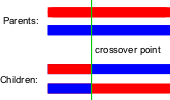
\includegraphics[width=\textwidth]{SinglePointCrossover}
    \caption{Single Point Crossover}
  \end{subfigure}
  ~
  \begin{subfigure}[b]{0.3\textwidth}
    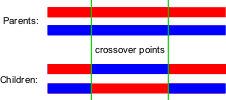
\includegraphics[width=\textwidth]{TwoPointCrossover}
    \caption{Two Point Crossover}
  \end{subfigure}
  ~
  \begin{subfigure}[b]{0.3\textwidth}
    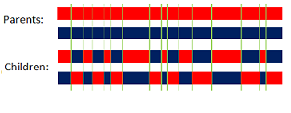
\includegraphics[width=\textwidth]{UniformCrossover}
    \caption{Uniform Crossover}
  \end{subfigure}
  \caption[Genetic Crossover Operations]{Genetic Crossover Operations. Images from Wikipedia}
  \label{fig:GeneticCrossover}
\end{figure}

Mutation is used to produce small, random changes in the genomes to maintain genetic diversity.
The mutation operation was chosen to be a simple bit flip in which a randomly chosen \verb+1+ or \verb+0+ in the geometry was flipped; for example \verb+001001010+ could be mutated to \verb+001001000+.
Generally the mutation rate is set very low (less than 2\%) in order to prevent the search for the solution to becoming simply a random search.
In this representation of the problem a mutation produces a very large change in the solution and the mutation rate was set even lower.

\subsection{Fitness Function}
\label{sec:FitnessFunc}
The fitness function defines the criteria for ranking solutions and probabilistically including them in the next generation.
The fitness function was chosen to count rate per mass of \iso[6]{Li}, provided that the geometry meet the total count rate criteria.
If it failed to meet the count rate criteria a zero fitness was returned \eqref{eqn:FitnessFun}.
\begin{align}
    \label{eqn:FitnessFun}
    f(\vec{x})
    = \begin{cases}
    0 & \text{if} \text{countRate}(\vec{x}) \leq \SI{2.5}{cps\per\nano\gram\iso[252]{Cf}} \\
    \text{countRatePerMass}(\vec{x})
    \end{cases}
\end{align}
Films that have excessive detector layers will be penalized by the normalization by the mass of \iso[6]{Li} that they contain, while favoring films that have the minimum number of detector layers that meet the count rate criteria and have a more effective utilization of the neutron flux which increase their count rate.

At this point it is instructive to make a note about the size of the solution space.
\autoref{tab:BitStringGeo} some of the these geometries are simple enough that the search space can be computed exhaustively.
\begin{table}
    \caption[Genome Bit String Geometries]{Bit String Simplified Geometry Descriptions}
    \label{tab:BitStringGeo}
    \centering
    \begin{tabular}{ c | c c}
     \toprule
     Genome Length&Slice Thickness&Possible Geometries \\
     \midrule
        5&2.54&31\\
        10&1.2700&1,023\\
        15&0.8467&32,765\\
        20&0.6350&1,048,575\\
        25&0.5080&33,554,431\\
        30&0.4233&\num{1.07E9}\\
        35&0.3629&\num{3.44E10}\\
        40&0.3175&\num{1.10E12}\\
    \bottomrule
    \end{tabular}
\end{table}
There are several salient features highlighted in \autoref{tab:BitStringGeo}.
For small genome lengths (less than 10) it is possible to exhaustively search the hypothesis space of possible solutions.
This is not possible for the larger genome lengths.
Therefore, efficient evaluation of the fitness function is necessary in order to evolve a reasonable number of solutions.
In addition the refinement in the details of the geometries increases linearly with the genome length while the size of the search space increases as $2^n$.
This suggest that a hybrid method of finding a basic geometry in a low search space and then preforming perturbations on that geometry will have a better performance than attempting to search the higher geometry solution space.

